As an aside from the primary work on fixed lag particle filtering for tracking, a short study has been made on inferring the intended destimation of a computer mouse cursor, as a component for aiding disabled computer user. A number of algorithms have been implemented and tested on a set of logged data.



\section{Algorithms}
The input to the algorithm is a series of logged cursor positions. Measurements are received asynchronously and consist of a time stamp and (x,y) coordinates. In addition, markers indicate when a click occurs.

Datasets have been logged in which a sequence of buttons appear on the screen, and users are instructed to click on them as quickly as possible. The purpose of the algorithm is to infer which button the users are intending to click on at each point in time. In the tests, only one button is ever present at once (making the inference task rather easy!), so a grid of phantom buttons is introduced, tiled over the screen. Models are devised which will allow calculation of a likelihood for each of the buttons in this grid. Thus a maximum likelihood (ML) or maximum a posteriori (MAP) choice can be made. The performance of the algorithms can be assessed by comparing the proportion of time during which the correct button is chosen.



\subsection{Nearest Neighbour}
The simplest conceivable algorithm for selecting a button is to pick that which is closest to the cursor at the given time instant. This most basic of schemes will be used as a benchmark against which to compare others. Such a scheme has a probabilistic interpretation, that the cursor position is normally distributed with mean at the target button and a fixed variance. This interpretation can be useful for calculating probabilities for each button, rather than just finding a ML or MAP choice.

\begin{equation}P(x_k|b_i) = \mathcal{N}(x_k|b_i, \sigma^2 I)\end{equation}
where $x_k$ is the $k^{th}$ measurement of the cursor position, $b_i$ is the $i^{th}$ button, $I$ the $2 \times 2$ identity matrix and $\sigma$ the standard deviation, a design parameter.

If we consider that the cursor position at every measurement is independent (clearly not true, but we are aiming for simplicity), then we can find the posterior probability of each button given some set of the measurements.

\begin{equation}
P(b_i|x_{1:k}) = \frac{P(b_i)\prod_{j=1}^{k}{P(x_j| b_i)}}{P(x_{1:k})}
\end{equation}

We assume a uniform prior over the buttons, although more sophisticated choices could be used if prior knowledge about the probaility of each button is known. The MAP choice of button is now that with the least mean square distance to the cursor over the measurements $x_{1:k}$, which accords with intuition. We need not necessarily use all the measurements for this calculation, but only those which lie in a window of fixed time length before the current time. The length of this window, $L$, is another design parameter.

\subsubsection*{Summary}
Pick the button which is closest to the cursor (on average).
Design parameters: Window length, $L$.



\subsection{Mean-Reverting Diffusion}
The cursor movement can be modeled as an Ornstein-Uhlenbeck process, a diffusion with a mean-reversion term. The cursor velocity is assumed to have two components, one random (Gaussian) and one deterministic which moves it towards the correct button.

\begin{equation}dx_t = \lambda (b_i - x_t)dt + \sigma dw_t\end{equation}
where $w_t$ is a Wiener process.

This may be solved analytically and discretised to give:

\begin{equation}P(x_{k+1}|x_{k}, b_i) = \mathcal{N} ( x_{k+1} | \mu_k, \gamma_k I)\end{equation}
where $x_k$ is the $k^{th}$, measurement made at time $t_k$, and:

\begin{equation}\mu_k = x_{k} + (b_i - x_k) (1-\exp(-\lambda (t_{k+1} - t_k)))\end{equation}
\begin{equation}\gamma_k = \sigma^2 \bigg (\frac{1-\exp(-2 \lambda (t_{k+1} - t_k))}{2 \lambda} \bigg )\end{equation}

$\sigma$ and $\lambda$ are design parameters.

As before, we can calculate the posterior probability given a set of measurements.

\begin{equation}
P(b_i|x_{1:k}) = \frac{P(b_i)P(x_1|b_i)\prod_{j=2}^{k}{P(x_j|x_{j-1}, b_i)}}{P(x_{1:k})}
\end{equation}

We assume a uniform prior over the buttons, and the starting point, $x_1$. The posterior for each button is thus proportional to the product of the transition probabilities given that button. As before, the length of the window used must be selected.

This algorithm has the advantage that when the cursor stops moving, the ML choice of button is that closest to the cursor, i.e. it reverts to a nearest neighbour scheme.

\subsubsection*{Summary}
Pick the button towards which the cursor is drifting.
Design parameters: Window length, $L$. Diffusion noise variance, $\sigma^2$. Drift coefficient, $\lambda$.



\subsection{Mean Bearing}
We can assume that the bearing moved along by the cursor between each consecutive pair of measurements is a random variable with a mean equal to the bearing of the target button.

\begin{equation}P(x_{k+1}|x_{k}) = \mathcal{N}(B_{x_k}(x_{k+1})|B_{x_k}(b_i), \sigma)\end{equation}
where $B_{a}(b)$ is the function which returns the bearing of $b$ from $a$. $\sigma$ is a design parameter.

As before, we can look at a set of measurements in a window as well as just one.

\subsubsection*{Summary}
Pick the button at which the path of the cursor is pointing.
Design parameters: Window length, $L$. Bearing noise variance, $\sigma^2$.



\subsection{Composite}
The bearing model works particularly poorly when the cursor is moving slowly, as it most often is, and thus does not have a clearly defined direction of travel. A composite algorithm has been implemented which uses the bearing model for high speeds and the mean-reverting diffusion model for low speeds.

Design parameters: Window length, $L$. Bearing noise variance, $\sigma_B^2$. Diffusion noise variance, $\sigma_D^2$. Drift coefficient, $\lambda$. Domain switching speed threshold, $S_T$.



\section{Results}
The algorithms were tested by running them on three data sets, those of subjects 1 (able-bodied), 14 (slightly impaired) and 21 (significantly impaired). As each measurement arrives, an estimate of the MAP button is made. We measure the proportion of time over which the correct button is chosen.

For three algorithms, the nearest neighbour (NN), mean-reverting diffusion (MRD) and mean bearing (MB), the design parameters were optimised by a simple grid method. The variance parameters do not affect the MAP choice of button, so the optimisation was only over 1 or 2 parameters, making is feasible.

For MRD, the best choice of diffusion coefficient was found to be $\lambda = 0.011-0.012$ for subjects 1 and 14 with a window length $L=0s$ (i.e. using only the latest measurement), and $\lambda = 0.004$ with $L=0.9s$ for subject 21.

For the NN algorithm, the optimum choice of window length was $L=0s$ for subjects 1 and 14, $L=0.5s$ for subject 21.

For the MB algorithm, the optimum choice of window length was $L=0.4s$ for subject 1, $L=0.5s$ for subject 14, $L=1.2s$ for subject 21.

For the Composite (Comp) algorithm, the parameters were set to the optimum values for each of the constituent algorithms. The threshold used was $S_T = 500 \text{pixel}/s$.

\begin{table}[!h]
\centering{\begin{tabular}{|c||c|c|c|c|}
\hline
 & \multicolumn{4}{|c|}{Proportion Correct by Algorithm (\%)} \\
\hline
Subject & NN & MRD & MB & Comp \\
\hline
1 & 44.4 & 49.4 & 14.9 & 42.4 \\
\hline
14 & 41.7 & 43.4 & 11.5 & 40.7 \\
\hline
21 & 55.4 & 55.9 & 7.4 & 54.9 \\
\hline
\end{tabular}}
\caption{Table showing percentage of time for which each algorithm picks the correct button, with optimised parameters.}
\end{table}

The best performance is obtained by the MRD algorithm, although the improvement over the NN algorithm is negligible for the impaired user, and is probably not worth the additional computation.

The MB algorithm performs very poorly according to the metric used. However, examining the posterior probabilities generally shows that the algorithm often identifies a likely cluster of targets in a wedge shape in front of the cursor. The correct target is often a member of the cluster, but is rarely picked out as the MAP choice. The videos of the algorithm in action demonstrate this well. A bearing-based approach may therefore have some use in combination with some other strategy.

Figure~\ref{fig:CursorTracking} shows a screenshot of a tracking algorithm in action. The circles represent the grid of phantom buttons. The real button is shown with a red circle. The shading of the circles represents the posterior probability of the button. The blue line is a trace of the cursor movement. The red cross indicates the button selected by the algorithm.

\begin{figure}[hbt]
\centering 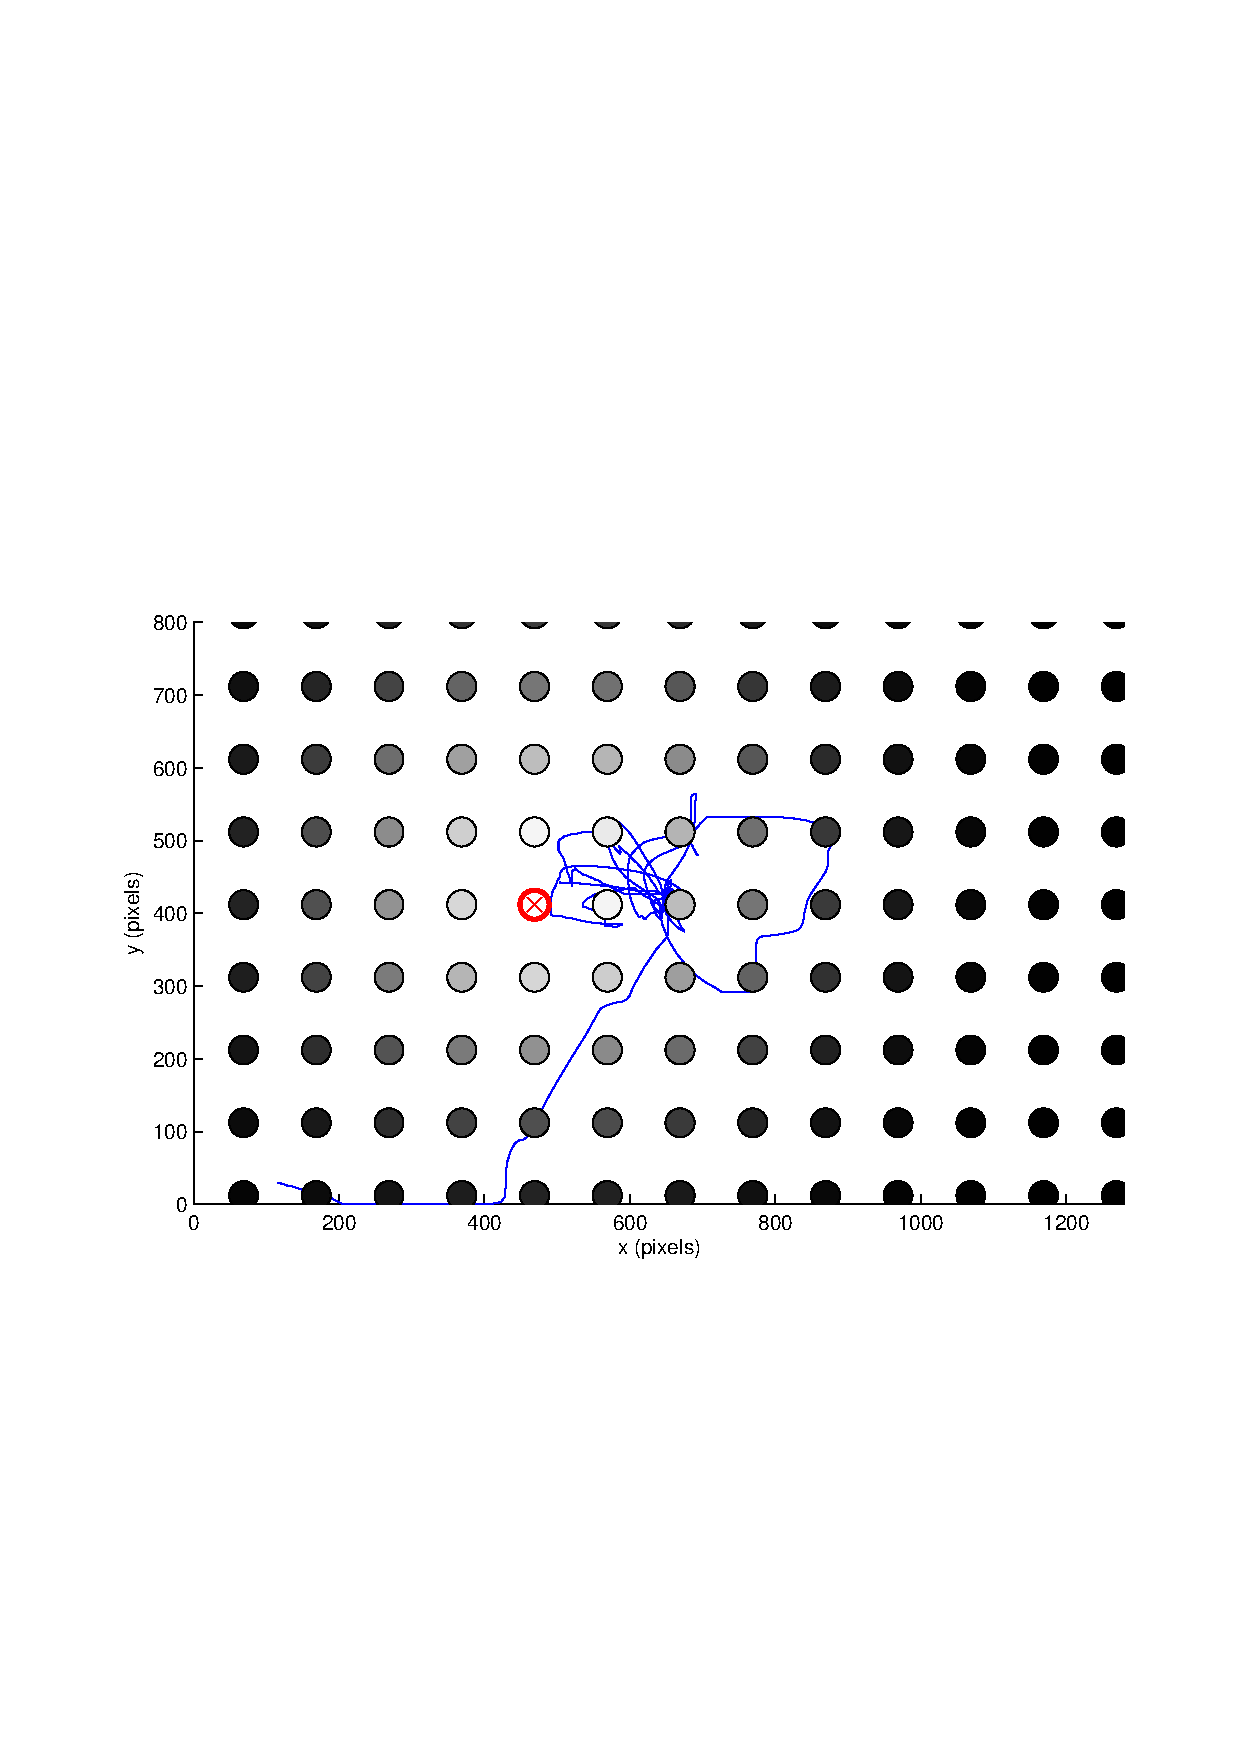
\includegraphics[width=0.9\textwidth]{MovieScreenshot.pdf}
\caption{A screen shot from the MATLAB-generated movies showing cursor trace, the grid of phantom buttons and their probabilities. See text for details.}
\label{fig:CursorTracking}
\end{figure}